\chapter{Prototype tests at IPHI}
\chaptermark{Prototype tests at IPHI}
\cleardoublepage

\minitoc

\section{Introduction}
\begin{refsection}
  \label{ch4:Introduction}

  \section{Preliminary tests of silicon detector}
  \subsection{IRMA}
  \cite{Chaumont1981}
  \begin{figure}[!ht]
	\begin{subfigure}{0.5\textwidth}
		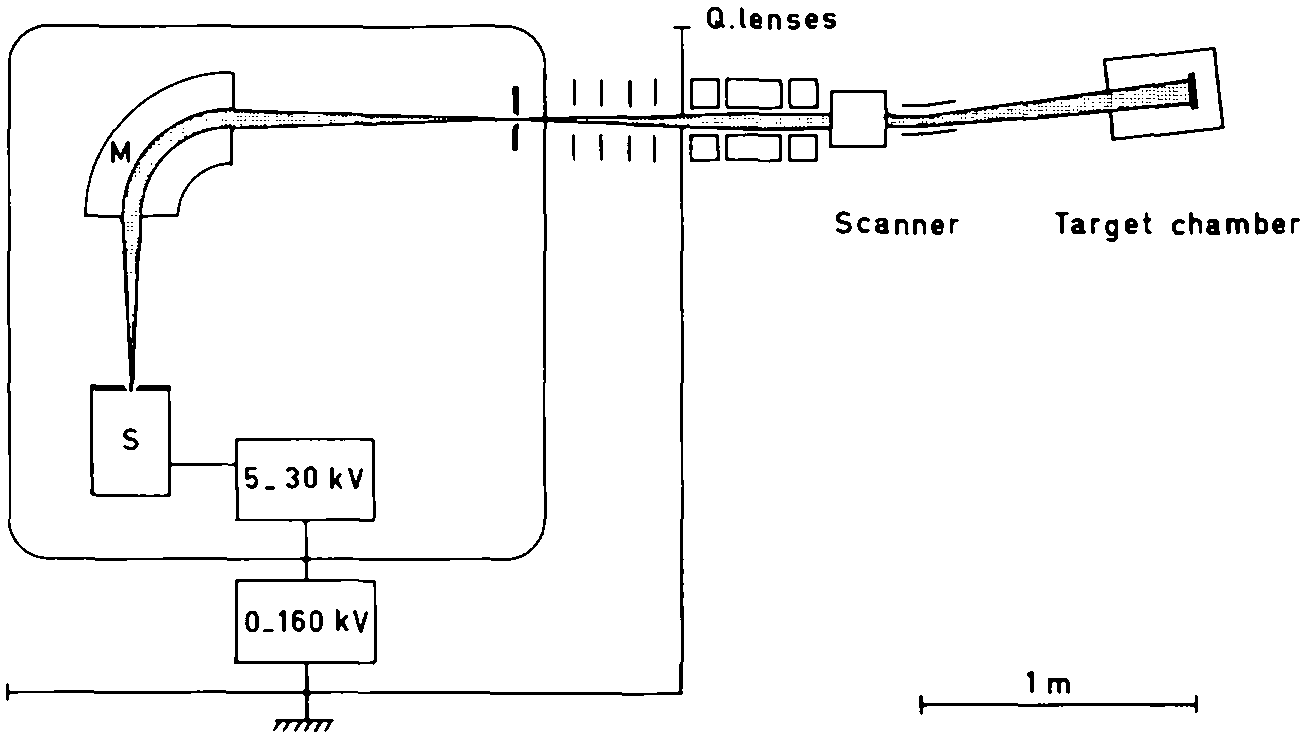
\includegraphics[width=\textwidth]{04_IPHI_Test/figures/fig000_IRMA01.png}
		\caption{}
		\label{}
	\end{subfigure}
	~
	\begin{subfigure}{0.5\textwidth}
		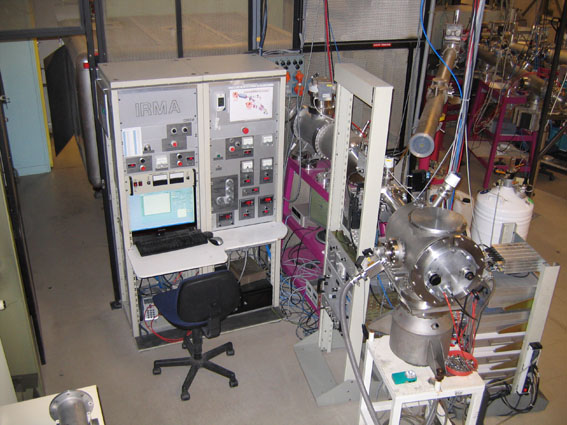
\includegraphics[width=\textwidth]{04_IPHI_Test/figures/fig000_IRMA02.jpg}
		\caption{}
		\label{}
	\end{subfigure}
	\caption[IRMA installation]{IRMA installation}
	\label{chap4:IRMA_facility}
\end{figure}

  \subsection{Test setup}
  \cite{advacam2019}
  \cite{Kraus2011}

  \begin{figure}[!ht]
	\begin{subfigure}[t]{0.5\textwidth}
		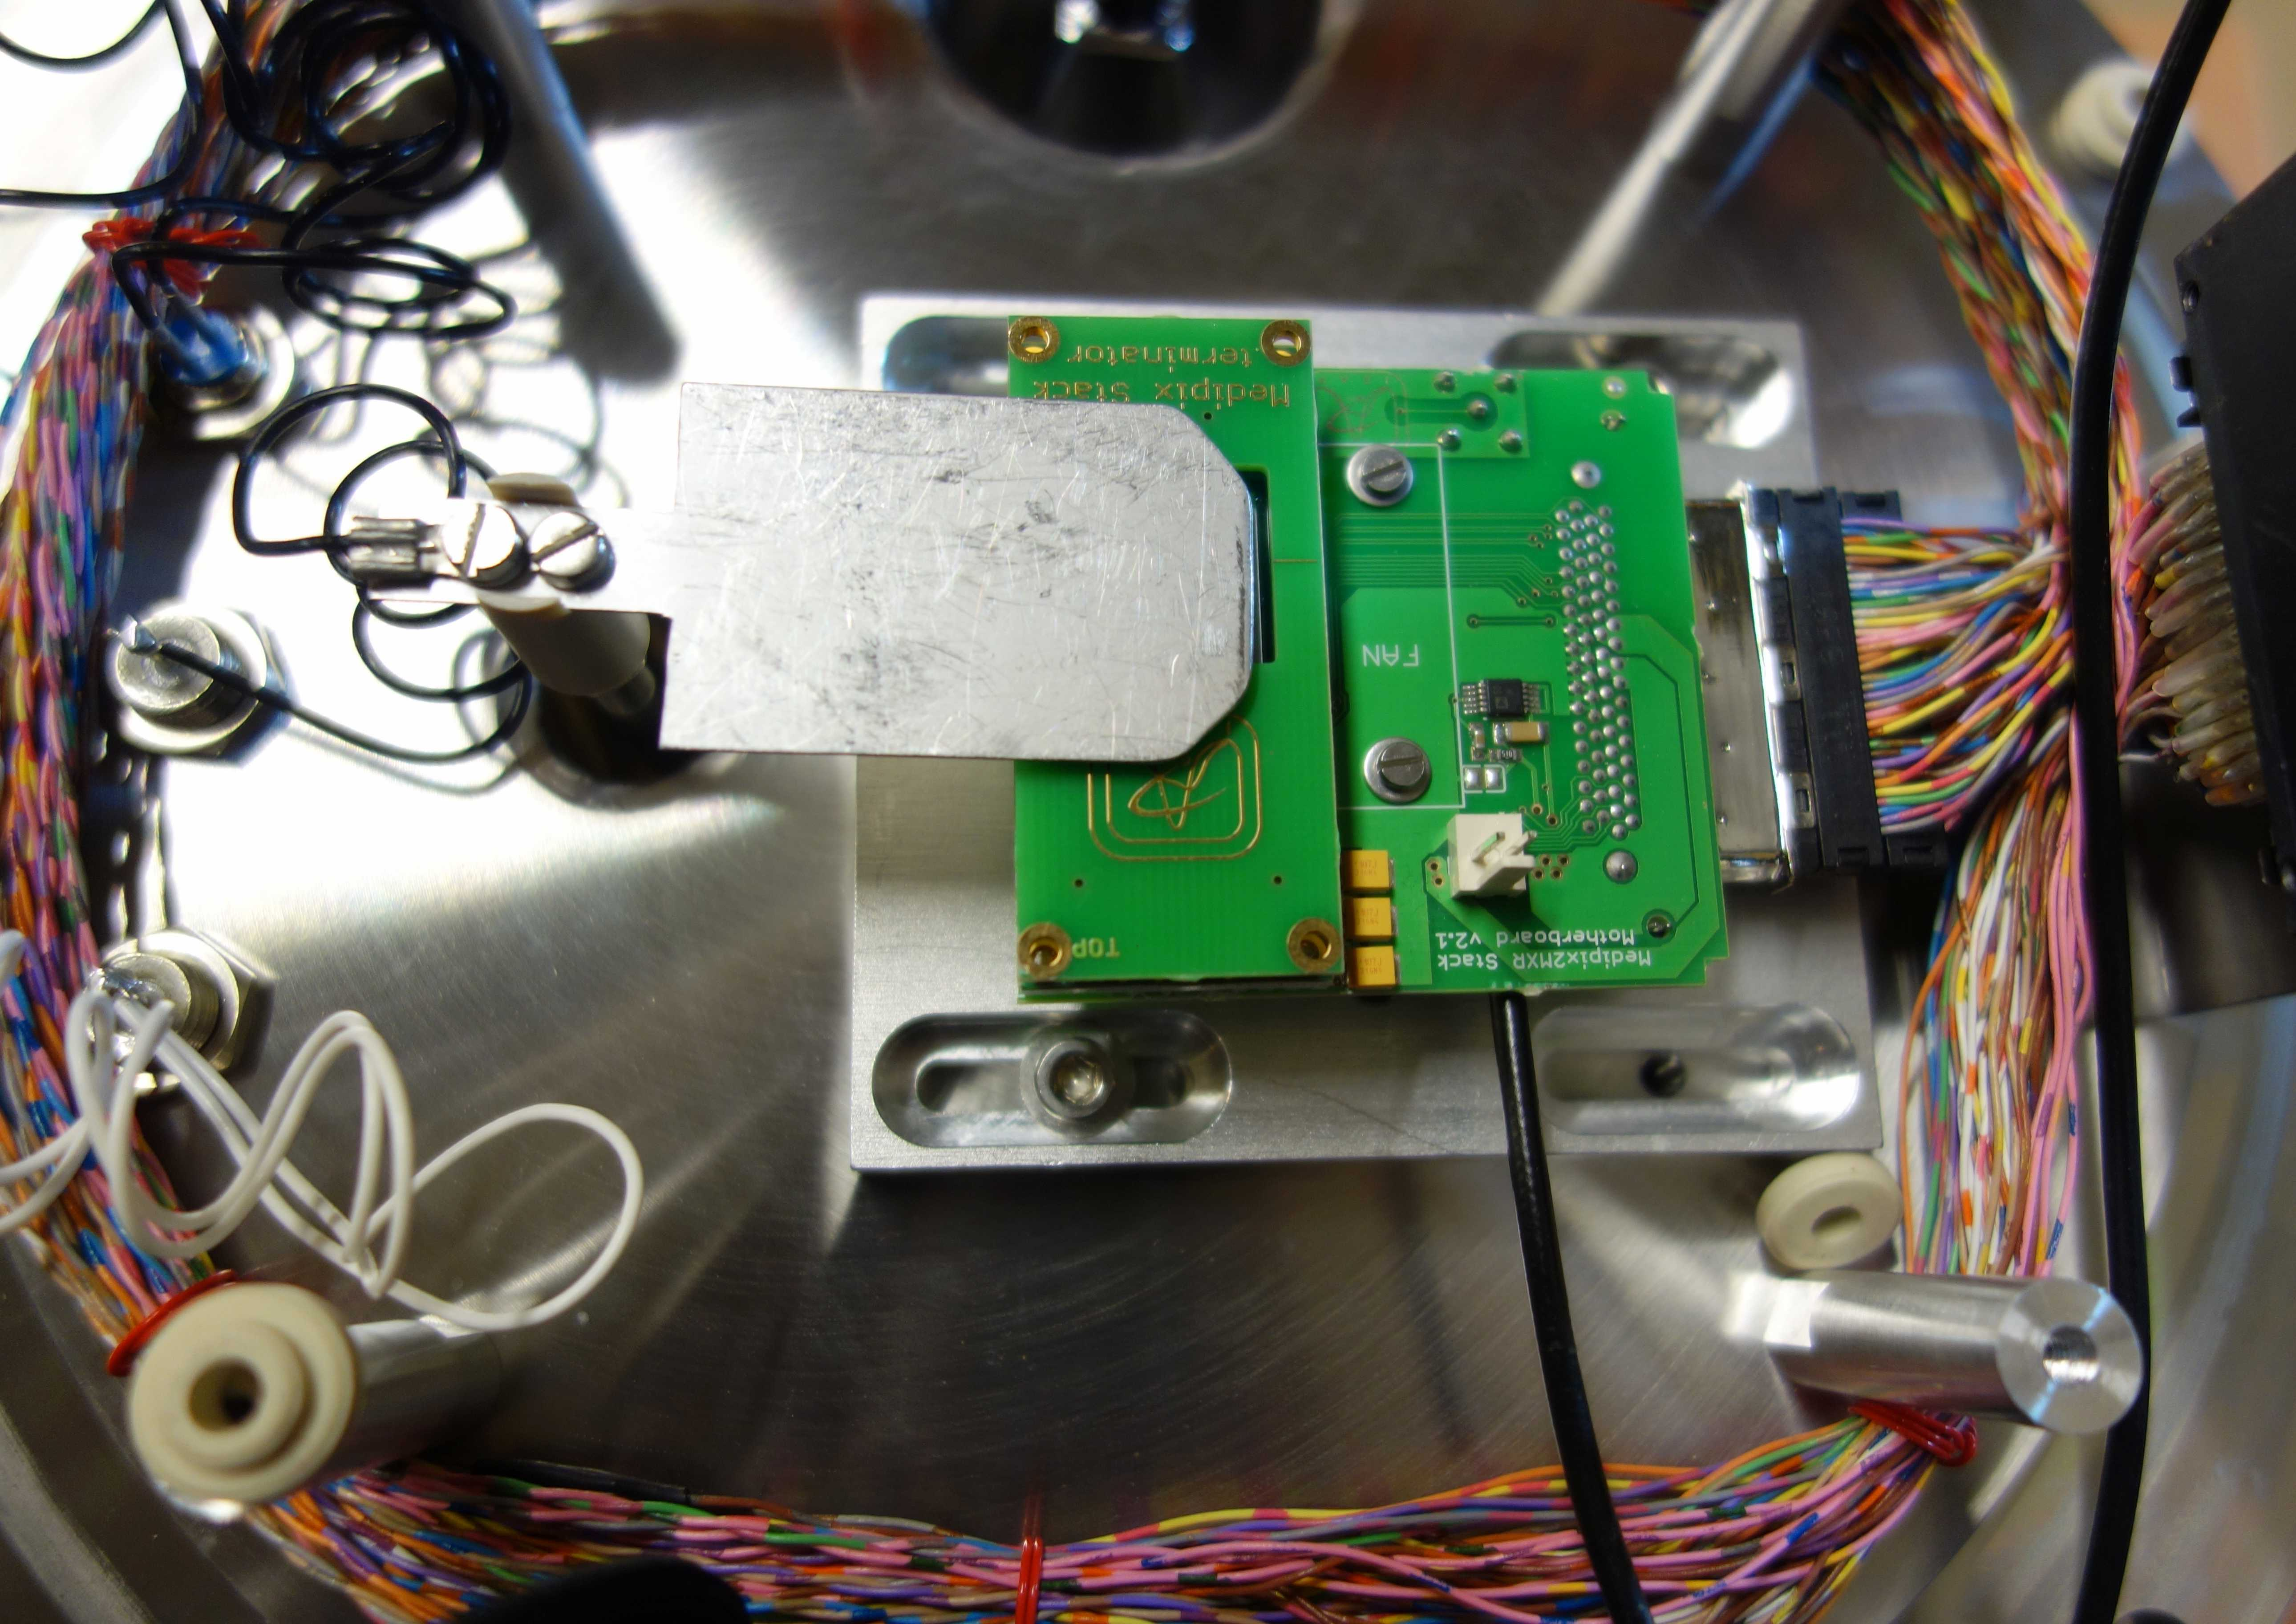
\includegraphics[width=\textwidth]{04_IPHI_Test/figures/fig000_IRMA_setup01}
		\caption{The TimePix chip is just behind the Faraday cup.}
		\label{}
	\end{subfigure}
	~
	\begin{subfigure}[t]{0.5\textwidth}
		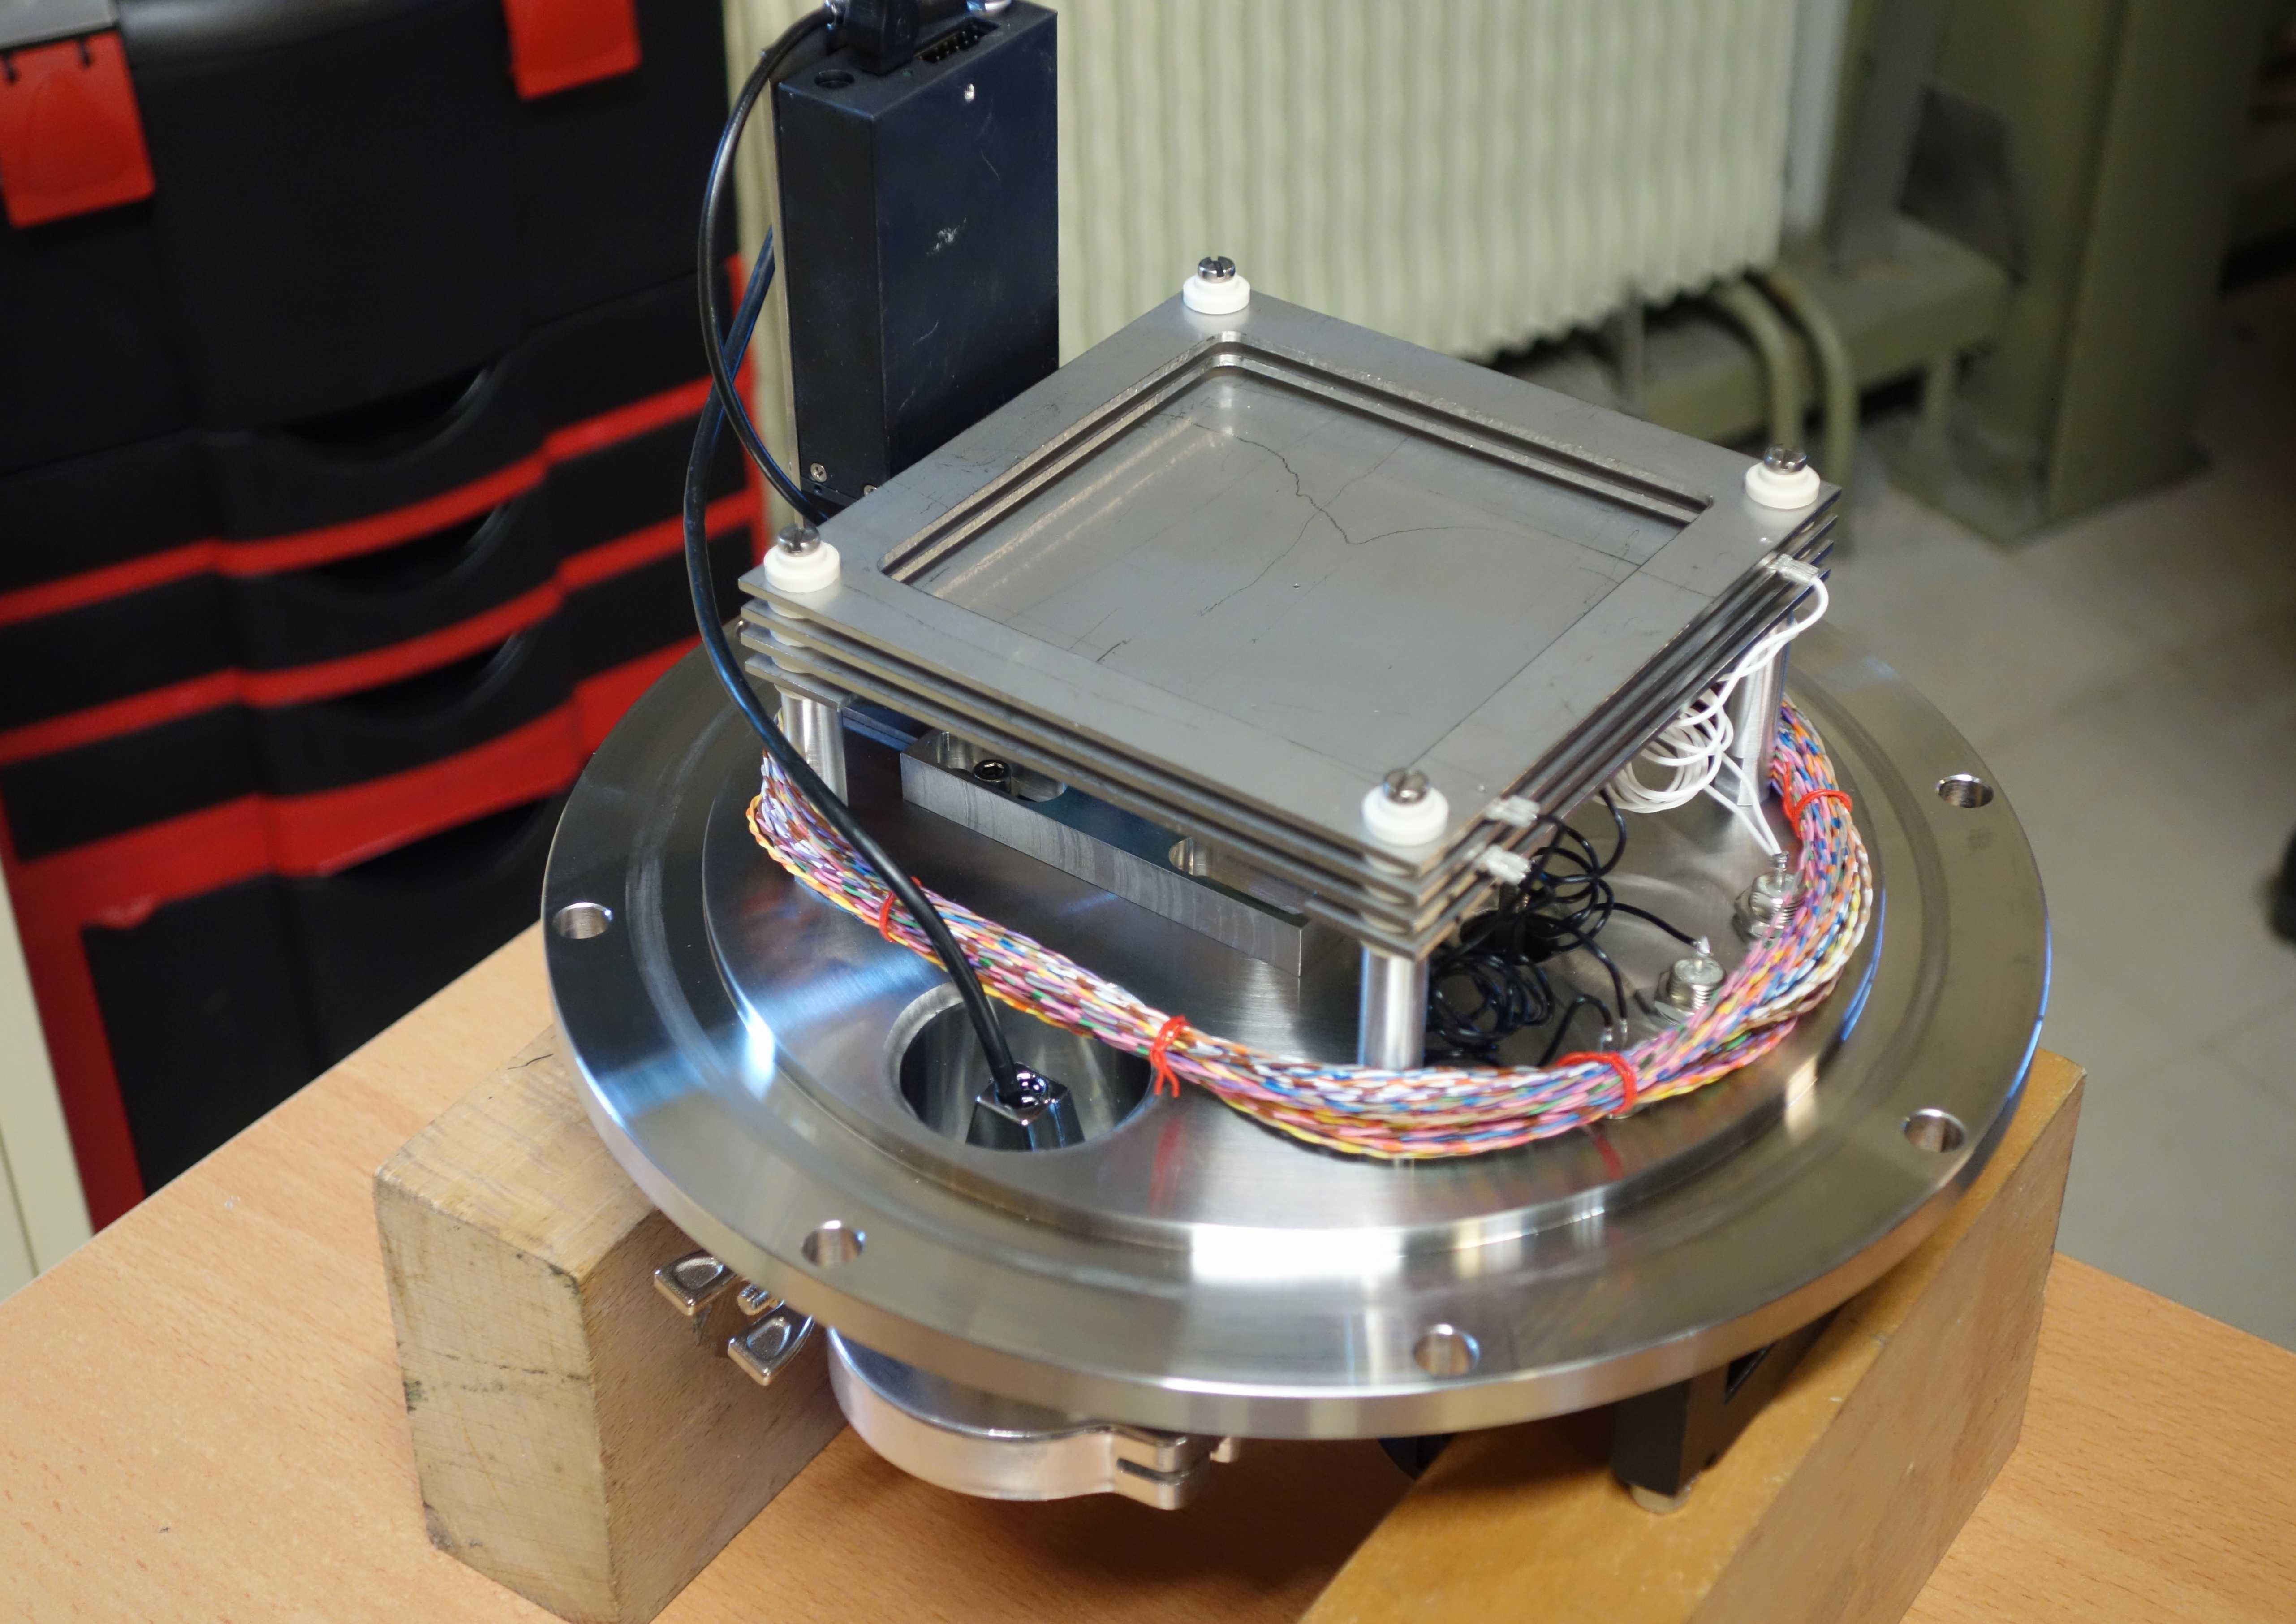
\includegraphics[width=\textwidth]{04_IPHI_Test/figures/fig000_IRMA_setup02}
		\caption{A plate with a drilled hole reduced the incoming current. The beam is scanned on the plate.}
		\label{}
	\end{subfigure}
	\caption[IRMA setup]{IRMA setup. A dedicated test bench has been developed for testing the TimePix chips.}
	\label{chap4:IRMA_setup}
\end{figure}

  \subsection{Results and limitations}

  \section{IPM design overview}
  \subsection{IPM}
  \subsection{MCP}
  \subsection{Camera}
  A vision system is necessary to record light from the phosphorus screen.
  A camera with a lens should be sufficient in our case.

  % Sensor
  Sensor is the core component of a camera so it's better to choose the sensor first with respect to the requirements.
  For our application high resolution is not mandatory, so pixels could be relatively big in order to increase light collection and dynamic range.
  Sony IMX249 fits well with these prerequisites. It's a consumer CMOS sensor with relatively big pixels and low noise.
  Its EMVA characteristics are summarized in the Table \ref{tab:IMX249} \cite{emva2010}.
  \begin{table}[!h]
  \centering
  \caption{Main features of the Sony IMX249 sensor}
  \label{tab:IMX249}
  \begin{tabular}{ll}
    \toprule
    Resolution           & 1936 (H) * 1216 (V)  \\
    Pixel size           & 5.86 $\mu m$         \\
    Sensor diagonal size & 13.4 mm (Type 1/1.2) \\
    Well capacity        & 32000 e-             \\
    Dynamic Range        & 70 dB                \\
    QE at 525 nm         & 70 \%                \\
    Electrons noise      & 6.8 $e^{-}$          \\
    ADC                  & 8, 10 or 12 bits     \\
    Max framerate        & 30 fps               \\
    \bottomrule
  \end{tabular}
\end{table}

  % Camera
  AlliedVision, Basler and FLIR propose several cameras based on the IMX249 sensor with different interfaces, features, form factors, prices and availability.
  We restricted our choice to GigE cameras since they allow long cable length and Power over Ethernet (PoE) which are quite useful features for an accelerator experiment.
  At the end we choose the FLIR Blackfly-PGE-23S6M-C \cite{blackfly2019}.

  % Lens
  The last step is the choice of a correct lens for the camera.
  Unfortunately lens suppliers doesn't provide full characteristics of their lenses, hence only the thin lens approximation has been considered.
  Distance from back of phosphorus screen to external air-side of viewport is 247mm. Active area radius of our MCPs is around 25mm thus magnification, with respect to a sensor size of 11.34 mm, should be at least 0.2268.
  Table \ref{tab:lens_magnification} shows magnification for several focal length. A focal length of 50 mm fits very well with our configuration.
  \begin{table}[!h]
  \centering
  \caption[Magnification for several common focal lengths]{Magnification for several common focal lengths, at a working distance of $247\,\mathrm{mm}$.}
  \label{tab:lens_magnification}
  \begin{tabularx}{1\textwidth}{lllllllll}
    \toprule
    Focal length ($\mathrm{mm}$) & $5$    & $15$    & $28$    & $35$    & $50$    & $75$    & $100$  & $150$   \\
    Magnification     & $0.02$ & $0.069$ & $0.127$ & $0.165$ & $0.255$ & $0.436$ & $0.68$ & $1.546$ \\
    \bottomrule
  \end{tabularx}
\end{table}

  Lenses with 50mm focal length are rather standard and commercially available at moderate cost. In addition these lenses have a large numerical aperture (or small F-number) so they provide a large photon capture efficiency.

  \subsection{Strips}
  \subsection{CARAMEL board and FASTER system}
  \cite{ddc316}\cite{caramel2013}\cite{faster2013}\cite{rhb2012}
  \subsection{Control System}
  The whole ESS Control System (CS) will rely on the EPICS (Experimental Physics and Industrial Control System) toolkit. The ESS CS team has specified its own EPICS standards to ensure the sustainability of the control system over the years. We will also test our IPMs in an accelerator that is EPICS compatible. Therefore, EPICS has some importance to our project and we tried to use it as much as possible for our prototypes. In this section we will briefly describe EPICS and how we have integrated our test bench.

  EPICS provides a set of tools and protocols to facilitate the integration of control system \cite{epics2019}. Originally developed for real-time systems, EPICS now supports many platforms. EPICS has become an open source project in 2004, since many laboratories and collaborations have contributed to EPICS.
  One of most important component of EPICS is the Channel Access (CA). In few words, it is a protocol that defines how the data are exchanged between clients and servers on a network. A server provides Processes Variables (PV) to clients. A PV is a useful data (for instance a current, a voltage or a temperature) associated with metadata (timestamp, units). A client can access and edit a PV value by knowing its name. In practice a server is often an hardware controlled by software, often called software Input / Output Controller (softIOC). A client is for instance an operator interface (OPI) which allows to view and modify the PV from one or more softIOCs.

  The whole system is almost fully compatible with the version 3.16 of EPICS base. The PointGrey GigE cameras are well supported by the AreaDetector module \cite{ad2019}. A custom plugin, developed by ESS, perform an gaussian fit on the profile every image. Raw images are saved into HDF5 files \cite{hdf5}. It allows to pack  various datasets together, for instance the raw IPM images with some beam information.
  Since all high voltage power supplies have their own SPCI Ethernet interface, thus a simple softIOC with StreamDevice\cite{streamdevice2019} was enough to control and monitor them.
  Three OPIs have been developed in order to control cameras, power supplies and geobrick. They run under BOY module of the ESS Control System Studio version 4.5. An Archiver Appliance records and saves slow process variables from the power supplies, the vacuum systems and the accelerator \cite{archiver2019}.

  \begin{figure}[!ht]
	\begin{center}
		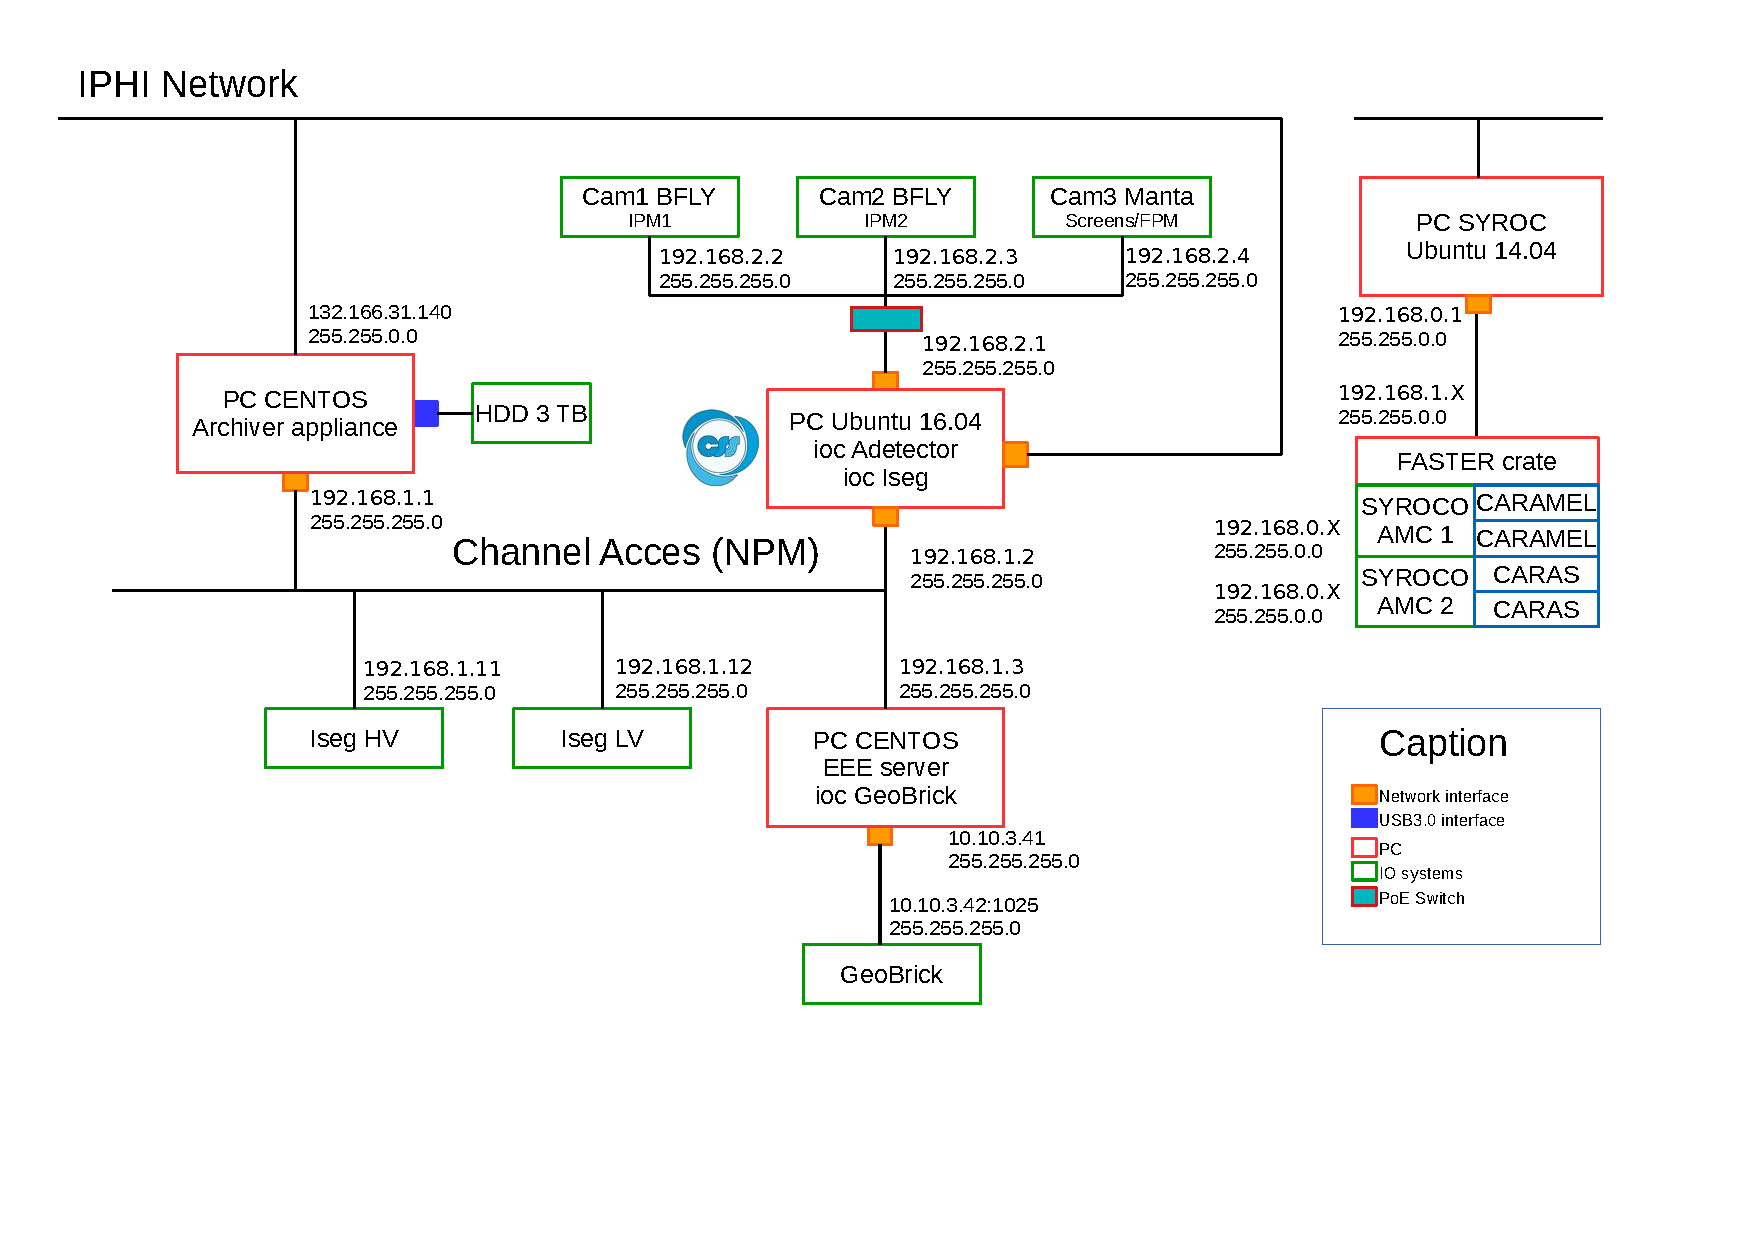
\includegraphics[width=\textwidth]{04_IPHI_Test/figures/fig000_EPICS_IPHI.pdf}
	\end{center}
	\caption[EPICS network setup during beam tests]{EPICS network setup during beam tests.}
	\label{chap4:EPICS_IPHI}
\end{figure}


  \subsection{Test bench}
  A test bench has been also developed in order to test the prototypes. The bench can be split into two different independent parts.

  The first part (upstream) tries to mimic the ESS LWU chamber on which two IPMs can be inserted. The idea is to be close to the ESS conditions in term of high voltages and electrical fields.
  The second part (downstream) offers one more IPM slot and two viewports for reference measurements in order to compare with the IPMs.

  Two solutions have been considered for the reference measurements, fluorescence profile monitor (FPM) and scintillating screens.

  The IPMs can be mounted independently in Y or X direction thanks to their design, thus it is even possible to measure the same profile direction with all three IPMs.

  \begin{figure}[!ht]
	\begin{center}
		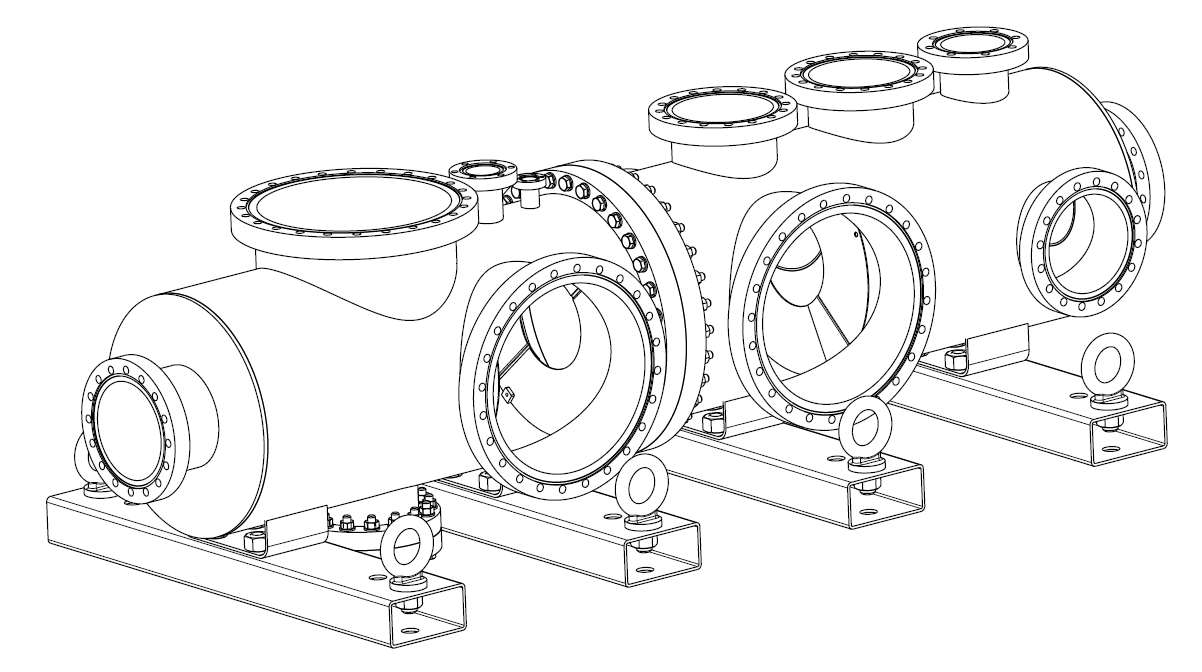
\includegraphics[width=\textwidth]{04_IPHI_Test/figures/fig000_Testbench.png}
	\end{center}
	\caption[IPM test bench]{IPM test bench. Left part is the LWU-like vessel
	while right part add more viewports for testing purposes.}
	\label{chap4:Testbench}
\end{figure}



  \subsection{Reference measurement}
  \section{IPHI test campaigns}
  \subsection{IPHI accelerator}
  IPHI is a high intensity linear proton accelerator located at CEA/Saclay.
  This project has been started in the late of 90's\cite{Beau2000} but protons were accelerated up to 3 MeV in April 2016\cite{Gobin2016}.

  Proton plasma is created by an electron cyclotron resonance source (ECR), and transported toward a radio frequency quadruple (RFQ) by a low energy beam transport line (LEBT).
  An iris assures a fine tuning of the current, and two solenoids focus and filter the plasma before the injection in the RFQ.
  Then, the protons are accelerated up to 3 MeV and bunched with a frequency of 352 MHz by the RFQ.
  A medium energy beam transport line (MEBT), downstream from the RFQ, contains focusing elements, steerers, dipole magnet and beam diagnostics.
  The dipole magnet can distribute the protons over two beam lines.

  The main line has a dedicated beam stop of 300 kW, allowing the commissioning of the accelerator at high intensity and duty cycle.
  The secondary line is more modular but restricted to lower intensity and duty cycle (few hundred Watts).
  This line is open for external user experiments.
  We were, with the nBLM team, one of the first experiments on the deviated line\cite{Senee:IPAC2018-TUPAF016}.

  Figure \ref{chap4:IPHI_view} shows schematic view of IPHI accelerator, and Table \ref{chap4:IPHI_carac} sums up difference between IPHI and ESS.

  \begin{figure}[!ht]
  \begin{center}
    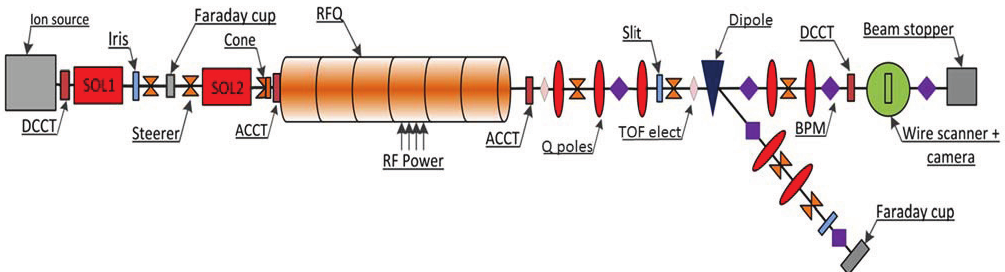
\includegraphics[width=\textwidth]{04_IPHI_Test/figures/fig000_IPHI_view.png}
  \end{center}
  \caption[Schematic view of IPHI accelerator]{Schematic view of the IPHI accelerator. The layout is almost up to date except that the slits have been removed. Our test bench was installed just after the last BPM on the deviated line.
    There is no other beam profiler measurement on this line.}
  \label{chap4:IPHI_view}
\end{figure}

  \begin{table}[!h]
  \centering
  \caption[Comparison between IPHI and ESS accelerators]{Comparison between IPHI and ESS accelerators.}
  \label{chap4:IPHI_carac}
  \begin{tabular}{lll}
    \toprule
                         & IPHI accelerator                                  & ESS accelerator                \\
    \midrule
    Energy               & $3\,\mathrm{MeV}$                                 & $2\,\mathrm{GeV}$              \\ \hline
    Max current          & $100\,\mathrm{mA}$                                & $62.5\,\mathrm{mA}$            \\ \hline
    Max pulse duration   & up to DC                                          & $2.86\,\mathrm{ms}$            \\ \hline
    Max pulse repetition & -                                                 & $14\,\mathrm{Hz}$              \\ \hline
    Vacuum range         & $5\cdot10^{-7}$ to $1\cdot10^{-8}\,\mathrm{mbar}$ & $1\cdot10^{-9}\,\mathrm{mbar}$ \\
    \bottomrule
  \end{tabular}
\end{table}
  
  \subsection{Setup}

  \section{Results}
  \subsection{Processing camera}
  \subsection{Processing strip}
  \cite{Brun1997,Antcheva2009}
  \subsection{Processing screen}
  \subsection{Beam current}
  \subsection{Beam position}
  \subsection{Beam size and space charge}
  \subsection{Detection limits}
  \subsection{Comparison size}
  \subsection{...}
  \subsection{Electron measurement}

  \section{Summary}
  \label{ch4:Summary}

  \cleardoublepage
  \section{Bibliography}
  \label{ch4:bib}
  \printbibliography[heading=subbibliography]

\end{refsection}